\newpage
\clearpage

\section{Desenvolvimento do Projeto}
\label{project}

Nos capítulos anteriores, analisamos como as Redes Neurais Convolucionais (CNNs) - Capítulo \ref{cnn} - provocaram mudanças significativas nas abordagens de segmentação, expandindo as possibilidades de obtenção de resultados mais precisos e melhorando o desempenho dos métodos convencionais de segmentação, conforme discutido no Capítulo \ref{segment}.

Entretanto, ainda existem questões não resolvidas relacionadas às potenciais melhorias que modificações específicas nas componentes destas redes podem proporcionar \citep{AsgariTaghanaki2021DeepReview}. Dentre esses componentes, particular atenção é dada às limitações das camadas de \textit{pooling} tradicionais \citep{Liu2019Multi-LevelNetworks, He2015SpatialRecognition}. Estas camadas têm duas tarefas principais: reduzir a dimensionalidade dos dados, a fim de diminuir a carga computacional do modelo, e, simultaneamente, preservar as informações mais relevantes, principalmente as espaciais.

Neste contexto, o objetivo primordial deste trabalho é propor uma nova técnica de \textit{pooling} para CNNs, com ênfase na segmentação semântica. A abordagem proposta visa manter as informações espaciais dos dados de entrada enquanto realiza a necessária redução de dimensionalidade algo que não ocorre com os métodos tradicionais de \textit{pooling}. Os resultados obtidos serão posteriormente comparados com aqueles produzidos pelos métodos de \textit{pooling} comumente utilizados.

Este capítulo trata detalhadamente dos materiais e métodos utilizados para a condução da pesquisa, discutidos na Seção \ref{project:matmet}. Além disso, a metodologia empregada para conduzir os experimentos e as avaliações será explorada em profundidade na Seção \ref{project:methodology}, enquanto a aplicação de métricas específicas para a avaliação dos resultados será discutida na Seção \ref{project:exp_result}. Finalmente, vale citar que nesse capítulo será possível encontrar uma apresentação detalhada do novo método de \textit{pooling} proposto e seu impacto na performance das redes de aprendizado profundo.

\subsection{Materiais e Métodos}
\label{project:matmet}
A seção de Materiais e Métodos tem como objetivo detalhar as tecnologias utilizadas durante a pesquisa, abordando a implementação de uma nova técnica como a camada de \textit{pooling} em modelos de segmentação semântica (Seção \ref{project:bpca}), os recursos tecnológicos e \textit{hardwares} empregados para dar suporte aos testes, validações e avaliações de desempenho dos modelos (Seção \ref{project:techard}), e, por fim, os conjuntos de dados utilizados, fundamentais para todo o desenvolvimento, tanto em pesquisas preliminares quanto na etapa de segmentação (Seção \ref{project:dataset}).

\subsubsection{Tecnologias e \textit{Hardware}}
\label{project:techard}
Um dos principais recursos tecnológicos utilizados neste trabalho é a linguagem de programação \textit{Python}. Esta linguagem interpretada de alto nível é amplamente reconhecida na comunidade científica, com uma vasta gama de bibliotecas disponíveis que facilitam o desenvolvimento de soluções tanto em aprendizado de máquina e redes neurais profundas, quanto em visão computacional \citep{Millman2011PythonEngineers, Perkel2015Programming:Python}.

Várias bibliotecas complementaram o \textit{Python} no desenvolvimento deste projeto, especialmente aquelas projetadas para auxiliar na implementação de soluções de visão computacional, aprendizado de máquina e redes neurais. Destas, destaco o \textit{TensorFlow} e \textit{Keras}, utilizados juntos como um \textit{framework} para modelar, treinar e testar redes neurais, bem como definir otimizadores, funções de custo e métricas de desempenho \citep{Geron2017Hands-onSystems, Chollet2021DeepPython}. O \textit{OpenCV}, uma biblioteca poderosa para o processamento de imagens e aplicações de visão computacional, também desempenhou um papel crucial na aplicação de filtros de imagens e na realização de testes manuais para afinar os métodos que utilizam aprendizado profundo \citep{Bradski2000TheLibrary.}. Adicionalmente, a biblioteca \textit{Numpy} foi fundamental para realizar cálculos matemáticos e manipulações matriciais \citep{Oliphant2007PythonComputing, VanDerWalt2011TheComputation}.

No que diz respeito ao \textit{hardware} empregado para a pesquisa e desenvolvimento deste projeto, os componentes de \textit{hardware}, tais como as placas de vídeo e os processadores, foram cruciais para o processamento de dados durante as fases de treinamento e validação dos modelos de aprendizado de máquina. Inicialmente, os ensaios foram realizados na plataforma de computação em nuvem Google Colab \citep{Bisong2019GoogleColaboratory}, que disponibilizava uma placa de vídeo Tesla T4 GPU e um processador Intel Xeon CPU. No entanto, devido à limitações de disponibilidade e considerações de custo financeiro, foi realizada a transição para um sistema físico equipado com um processador Intel Core i9-12900F CPU e uma placa de vídeo NVIDIA RTX 4090 GPU, o qual foi considerado para todos os resultados e testes descritos no presente trabalho.

Por fim, é importante ressaltar que todos os métodos desenvolvidos neste projeto com o objetivo de realizar a segmentação semântica serão disponibilizados no repositório Github do autor\footnote{Perfil Github do autor - \url{https://github.com/Lucs1590}}, em conformidade com a licença Apache v2.0 \citep{Licenses}. A intenção é fomentar o crescimento acadêmico e de pesquisa, assim como facilitar futuras melhorias no campo de segmentação com o uso de camadas de \textit{pooling} personalizadas, como a camada BPCAPooling, que é detalhada na Seção \ref{project:bpca}.


\subsubsection{\textit{Block-based Principal Component Analysis Pooling} (BPCA Pooling)}
\label{project:bpca}

Apresentado como uma variação do método convencional do Principal Component Analysis (PCA) no trabalho \cite{Salvadeo2011}, o BPCA propõe um método que inicialmente foi utilizado para a extração de características de imagens relacionadas a trabalhos de reconhecimento de face, propondo um método de extração que trouxesse à análise menor custo computacional, redução de dimensionalidade e uma geometria de hiperespaço que fosse mais intuitiva, destacando o diferencial de que com esse método fosse possível preservar a espacialidade da informação.

O método proposto opera por meio da subdivisão de uma imagem em blocos $k \times k$, em que os blocos geralmente possuem tamanhos iguais (por exemplo, $3 \times 3$, $8 \times 8$, etc.). Em seguida, o PCA é aplicado a cada um desses blocos subdivididos. Consequentemente, cada bloco $k \times k$ passa a ter um tamanho reduzido, contendo apenas um subconjunto de pixels com $r$ características (o mesmo numero de blocos). Esse processo pode ser visualizado através da Figura X.

É importante ressaltar que o BPCA não é uma simples combinação linear de amostras distintas. Em vez disso, ele cria uma representação organizada, formada por pequenos blocos do mapa de características original usado como entrada. O BPCA incorpora o PCA para realizar o mapeamento não supervisionado que minimiza o erro quadrático médio entre a entrada original e a representação projetada.

Considerando os parágrafos anteriores e o fato de que as camadas de pooling são aplicadas com sucesso nas redes convolucionais com o objetivo de reduzir a dimensionalidade dos dados \cite{Paul2019DimensionalityPooling}, a partir do presente trabalho, propõe-se a utilização dessa técnica não para a tarefa de extração de características, mas como uma camada de pooling que contenha o benefício de preservar a espacialidade da informação entre as camadas convolucionais.

A camada de pooling adota o processo original do BPCA, que extrai as principais informações de cada bloco, reduzindo a dimensionalidade dos dados e preservando características relevantes. Além disso, o método foi aprimorado por meio da normalização dos blocos usando média ($\mu$) e desvio padrão ($\sigma$). Em seguida, é aplicada a decomposição em valores singulares (SVD) para extrair os componentes principais ($\text{{pca\_components}}$) que realizam a transformação dos blocos por meio da projeção nesses componentes selecionados. Como resultado, obtém-se um mapa de características reduzido em tamanho, mas que preserva a informação essencial ao concatenar os blocos transformados.

A representação matemática do processo realizado pela camada de pooling BPCAPooling pode ser descrita pela seguinte equação:

\[
\text{{BPCAPooling}}(x) = \text{{reshape}}\left(\text{{SVD}}\left(\frac{{x - \mu}}{{\sigma}}\right) \cdot \text{{pca\_components}}\right),
\]
onde $x$ representa o mapa de características de entrada, $\text{{reshape}}$ reorganiza os blocos transformados em uma estrutura de saída adequada, $\text{{SVD}}$ denota a decomposição em valores singulares dos blocos normalizados, $\mu$ é o vetor médio dos blocos extraídos, $\sigma$ é o vetor de desvio padrão dos blocos extraídos, e $\text{{pca\_components}}$ é uma matriz que contém os primeiros componentes principais selecionados.

Essa formulação matemática descreve o processo de pooling realizado pela camada BPCAPooling, que extrai informações relevantes dos blocos de entrada, reduzindo sua dimensionalidade e preservando características importantes para o aprendizado eficiente da rede neural convolucional.

\paragraph{Funcionamento como \textit{Pooling}}

\paragraph{Formula e Complexidade}
Dentre os métodos disponíveis para realizar a tarefa de segmentação panóptica de componentes visuais, destaca-se que serão realizados testes a partir dos modelos disponibilizados pela biblioteca \textit{Detectron2} \cite{detectron2}, seguindo também a formatação inicial proposta por Kirillov \textit{et al.} \cite{Kirillov2019a}, a qual era composta por um modelo de Mask R-CNN (Seção \ref{instance:mask}) para realizar a parte de segmentação de instâncias e o modelo de FCN (Seção \ref{semantic:FCN}) para realizar a segmentação semântica.

Todavia, haja vista o resultado esperado nesse trabalho, vide a Seção \ref{project:expres}, para as tarefas de segmentação panóptica com o uso de partes, diferente das abordagens de estruturas que possuem apenas as tarefas de segmentações de instâncias e semântica, seja de modo compartilhado, unificado, com conexões ou cascata, como demonstradas na Figura \ref{project:method:fig:1}, a segmentação de partes cientes necessita, também, de uma parte voltada para a segmentação das partes de objetos classificados como \textit{thing} ou \textit{stuff}, como demonstrado na Figura \ref{project:method:fig:2}, a qual representa uma estrutura voltada para a segmentação panóptica de modo unificado (segmentação semântica e de instância) e outra para a segmentação de partes cientes. Sendo assim, também será testada a estrutura desenhada por de Geus \textit{et al.} \cite{DeGeus2021}, a qual é composta por um modelo de segmentação panóptica (DLv3-ResNeSt269 \& DetectoRS) juntamente com um modelo responsável por realizar uma segmentação de partes (BSANet).

\begin{figure}[H]
    \centering
    \caption{Metodologias de rede para segmentação panóptica.}
    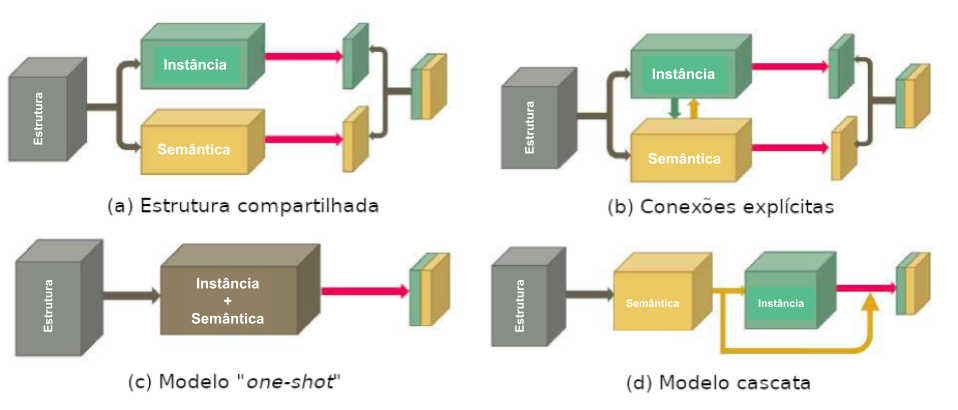
\includegraphics[width=1\textwidth]{recursos/imagens/proposal/model_methodologies.png}
    \label{project:method:fig:1}

    Fonte: retirado e adaptado de \cite{Elharrouss2021}.
\end{figure}

\begin{figure}[H]
    \centering
    \caption{Estrutura exemplificando metodologia para segmentação \textit{Part-Aware}.}
    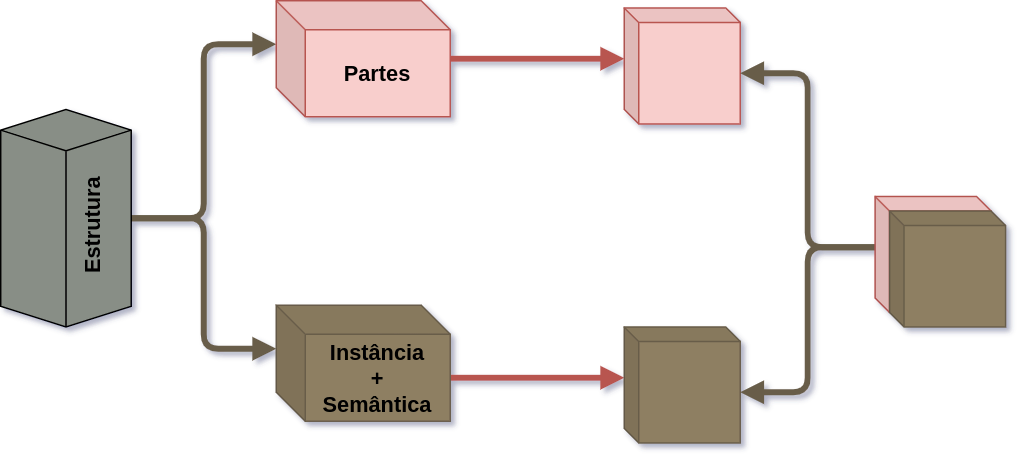
\includegraphics[width=4in]{recursos/imagens/proposal/estrutura.png}
    \label{project:method:fig:2}

    Fonte: do próprio autor.
\end{figure}

\subsubsection{Conjuntos de Dados}
\label{project:dataset}

Os conjuntos de dados selecionados para esta pesquisa são essencialmente de duas categorias distintas. Dois deles - CIFAR100 e Food-101 - foram empregados especificamente para o treinamento, teste e validação voltados exclusivamente à classificação de imagens \citep{Krizhevsky2009LearningImages, Bossard2014Food-101Forests}.

Nessa configuração, os modelos de classificação foram treinados para atribuir um rótulo a cada imagem, identificando o objeto de interesse sem foco na sua localização ou delimitação por caixas. Em outras palavras, o objetivo foi reconhecer a presença de um objeto em particular na imagem inteira, sem segmentar ou isolar essa entidade \citep{Viitaniemi2008TechniquesSegmentation}.

Por outro lado, um terceiro conjunto de dados - que será detalhado na Seção \ref{project:dataset:pets} - foi preparado especificamente para treinar e validar modelos de segmentação semântica. Este conjunto de dados inclui máscaras que mapeiam a localização dos objetos de interesse em todos os pixels da imagem de entrada.

O emprego desses conjuntos diversificados de dados permite comparar e contrastar a eficácia de diferentes abordagens de segmentação e classificação no campo da visão computacional. Também permite avaliar como esses diferentes métodos respondem a variações nas características dos dados.

As Seções \ref{project:dataset:cifar} e \ref{project:dataset:food101} a seguir detalharão mais apropriadamente os conjuntos de dados utilizados para os experimentos de classificação, e descreverão como foram utilizados no escopo desta pesquisa.

\paragraph{\textit{Oxford-IIIT Pet}}
\label{project:dataset:pets}

\paragraph{CIFAR 1O0}
\label{project:dataset:cifar}

\paragraph{\textit{Food}-101}
\label{project:dataset:food101}



Em relação ao conjunto de dados, por esse trabalho fazer uso da segmentação \textit{Part-Aware Panoptic Segmentation} proposta em \cite{DeGeus2021}, sendo que esta é uma nova abordagem, vale dizer que a quantidade de conjuntos de dados ainda é escassa, principalmente quando se trata de trabalhos voltados para uma área em específico, como a odontológica.

Todavia, no presente trabalho serão utilizados tanto conjuntos de dados que são mais generalistas, mas são voltados para a segmentação panóptica, quanto conjuntos de dados voltados para a parte odontológica, os quais precisarão ser anotados de modo a estarem adaptados para o seu uso em bases de treino e teste.

Quanto aos conjuntos de dados mais generalistas vale dizer que há algumas estratégias e justificativas para o seu uso, as quais serão descritas na Seção \ref{project:transf}, entretanto, dentre os conjuntos de dados escolhidos, destacam-se PASCAL \textit{Panoptic Parts} e \textit{Cityscapes Panoptic Parts}, sendo que os estes foram desenvolvidos pelos autores que abrolharam a segmentação panóptica com uso da técnica \textit{Part-Aware} \cite{DeGeus2021}.

O conteúdo dos conjuntos PASCAL \textit{Panoptic Parts} e \textit{Cityscapes Panoptic Parts} foram criados a partir dos conjuntos de dados \cite{everingham2010pascal} e \cite{Cordts2016}, sendo que o conteúdo do primeiro está voltado para pessoas, animais, veículos e cenas em locais fechados, quando o segundo conta com cenas de cidades, respectivamente, os quais são exemplificados na Figura \ref{project:dataset:fig:1}.

\begin{figure}[H]
   \caption{Imagens originais e anotadas dos \textit{datasets} para \textit{Part-Aware Panoptic Segmentation}.}
   \centering
   \label{project:dataset:fig:1}
    \begin{subfigure}[t]{0.45\textwidth}
        \centering
        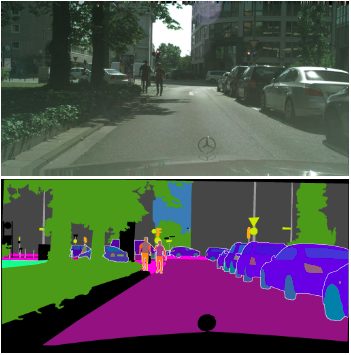
\includegraphics[height=2.5in]{recursos/imagens/proposal/city.png}
        \caption{Imagem original e anotada do \textit{Cityscapes Panoptic Parts}, respectivamente.}
        \label{project:dataset:fig:1.1}
    \end{subfigure}%
    ~ 
    \begin{subfigure}[t]{0.45\textwidth}
        \centering
        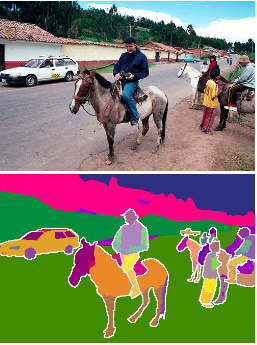
\includegraphics[height=2.5in]{recursos/imagens/proposal/pascal.png}
        \caption{Imagem original e anotada do PASCAL \textit{Panoptic Parts}, respectivamente.}
        \label{project:dataset:fig:1.2}
    \end{subfigure}%

    Fonte: retirado e adaptado de \cite{Lin2016}.
\end{figure}


Os conjuntos criados por \cite{DeGeus2021}, os quais contemplam segmentação \textit{Part-Aware}, quando relacionado ao \textit{Cityscape Panoptic Parts}, vale dizer que este possui 2975 imagens para treino e 500 para validação, totalizando em 3475 imagens dispostas em resolução de 1024×2048. Por sua vez, o PASCAL \textit{Panoptic Parts} possui 4998 imagens para treino e  5105 imagens para validação, as quais estão em resoluções de 387×470, totalizando à disposição de 10103 imagens.

Por fim, ainda há a disposição do conjunto de dados de partes, do qual se cita \textit{PartNet} \cite{mo2019} e \textit{PartImageNet} \cite{He2021}, sendo que o primeiro abrange a anotação de 573585 partes de instâncias, realizando a cobertura de 24 categorias de objetos, as quais também podem ser úteis para agregar ao projeto. Já o segundo, por ter sido criado com base no trabalho desenvolvido por \cite{DeGeus2021}, encontra-se disponível para o exercício das redes panópticas \textit{part-aware}, com 158 classes e por volta de 24000 imagens, visto que a fonte das imagens anotadas é o projeto \textit{ImageNet}.

Quanto aos conjuntos de dados comentados anteriormente que estarão dispostos para o meio odontológico, vale citar que esses não possuem uma anotação com classes de partes, as quais se fazem \textit{mister} para a aplicação panóptica com uso de \textit{Part-Aware}, todavia vale destacar que temos uma parceria da Faculdade de Odontologia de Araraquara (FOAr) - UNESP, a qual terá com líder o Prof. Dr. Osmir Batista de Oliveira Júnior, de modo que estudantes e especialistas da área realizem as anotações, bem como a disponibilização, de 5000 imagens de fotografias odontológicas, de modo a contribuírem para o projeto.

Além das fotografias cedidas pela parceria, vale destacar que alguns conjuntos de dados serão utilizados com o intuito de agregar em volume de imagens odontológicas, dos quais, cita-se o conjunto de dados desenvolvido por You \textit{et al.} \cite{You2020}, o qual possui 886 anotadas, o conjunto desenvolvido por Hyttinen \textit{et al.} \cite{Hyttinen2020}, com 316 imagens, sendo que 215 dessas imagens possuem uma anotação inicial e, por fim, o conjunto de dados disponível no \textit{website} da \textit{Dental Care}\footnote{\textit{Website \textit{Dental Care}} – \url{https://www.dentalcare.com/en-us/research/media-library}}, o qual cede 839 imagens odontológicas como cortesia para estudos e desenvolvimento científico. O objetivo é que todas essas 1370 imagens sejam agregadas à \textit{pipeline} de anotação e ao conjunto disponibilizado pela parceria, de modo a se tornarem úteis para a construção do modelo proposto no presente trabalho. Exemplos dos conjuntos de dados citados podem ser observados na Figura \ref{project:dataset:fig:2}.

\begin{figure}[H]
    \centering
    \caption{Exemplo de imagens dos conjuntos de dados odontológicos.}
    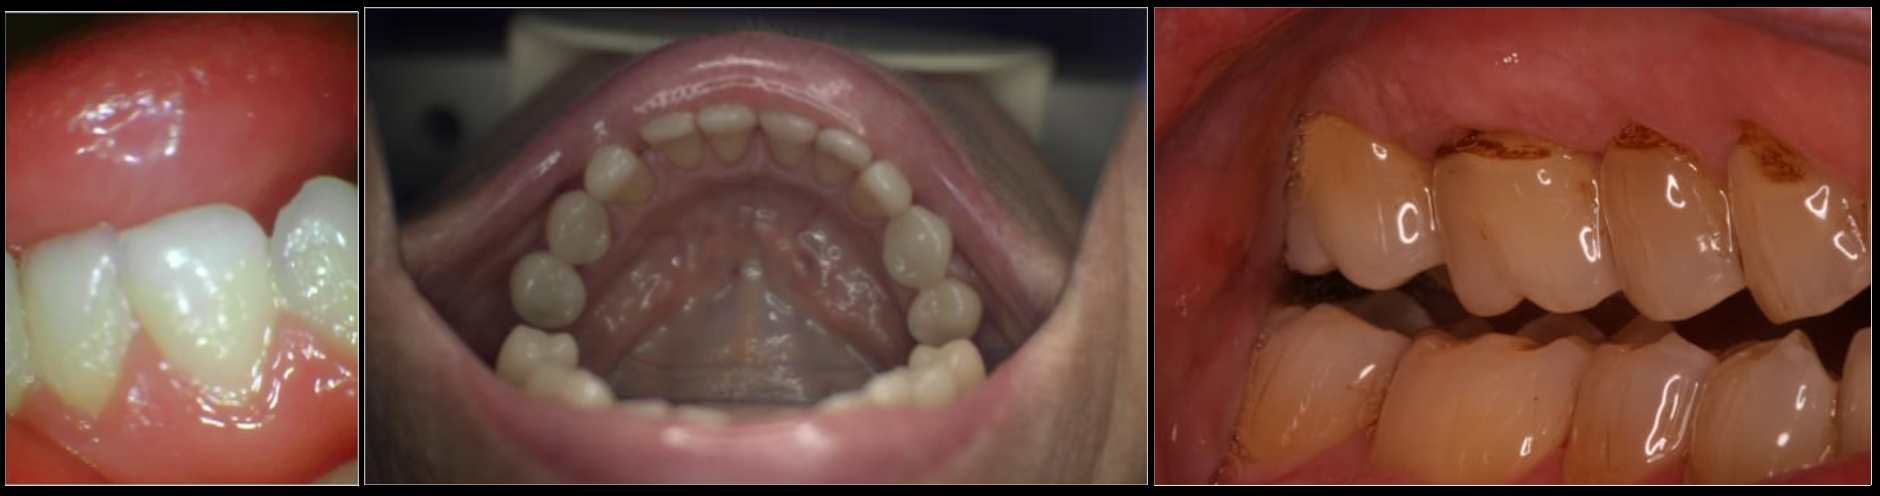
\includegraphics[width=1\textwidth]{recursos/imagens/proposal/image_odonto_dataset.png}
    \label{project:dataset:fig:2}

    Fonte: retirado e adaptado de \cite{You2020, Hyttinen2020} e \textit{Dental Care}, respectivamente.
\end{figure}

\subsection{Metodologia}
\label{project:methodology}
Nesta Seção, será descrito quanto à metodologia adotada para os experimentos a serem realizados, de modo a conquistar os objetivos propostos no presente trabalho. Na Seção \ref{proposal:transf} será detalhado sobre o processo de transferência de aprendizado a ser realizado no conjunto de dados, na Seção \ref{proposal:pcapooling} se discorrerá sobre o processo de alteração na camada de \textit{pooling} dos modelos e, finalmente, na Seção \ref{proposal:avaliation} será descrito o método de avaliação escolhido para a submissão dos modelos. Em resumo, o processo esperado resume-se na Figura \ref{project:methodology:fig:1}.

\begin{figure}[H]
    \centering
    \caption{\textit{Pipeline} do presente trabalho.}
    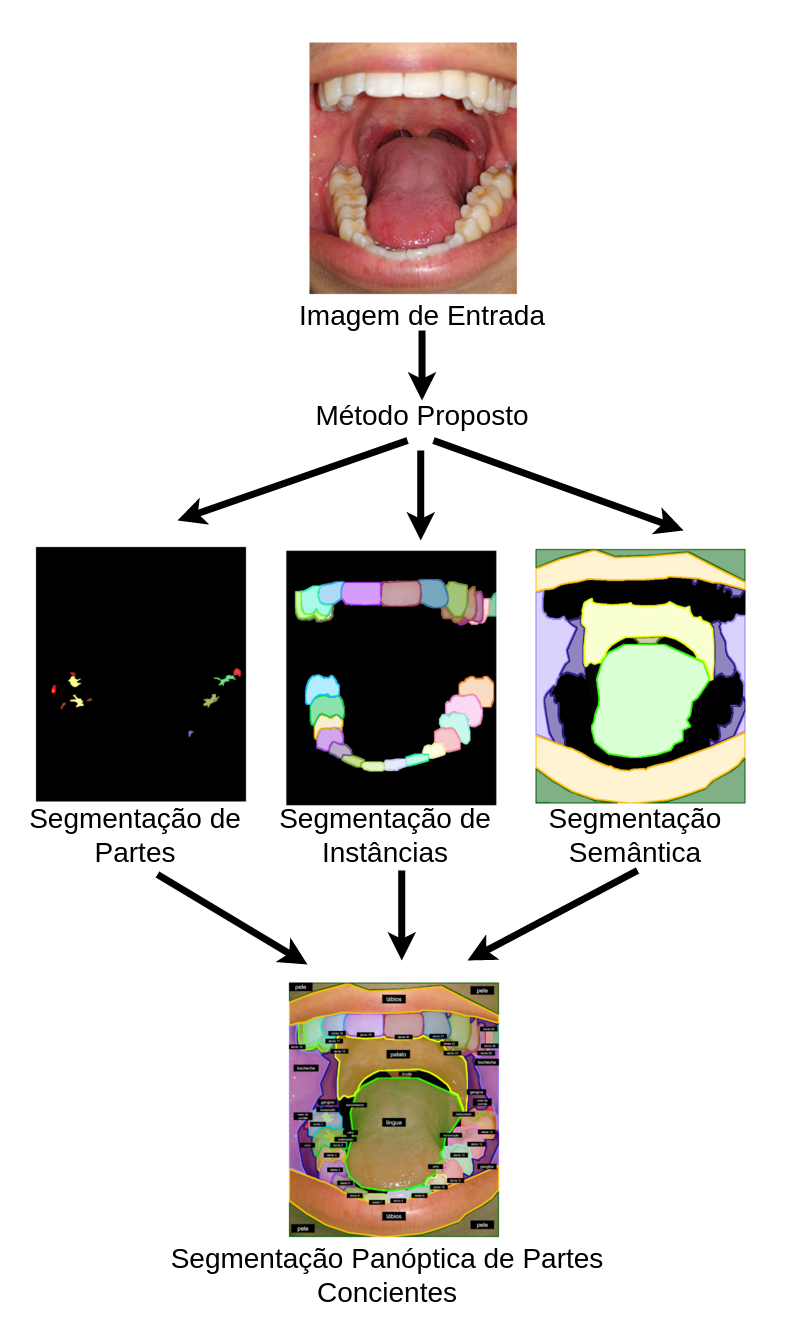
\includegraphics[width=0.7\textwidth]{recursos/imagens/proposal/full_diagram.png}
    \label{project:methodology:fig:1}

    Fonte: do próprio autor.
\end{figure}

\subsubsection{Transferência de Aprendizado}
\label{proposal:transf}
Tendo em vista que os conjuntos de dados na área odontológica preparados para a aplicação de segmentação panóptica com o uso da técnica \textit{Part-Aware} são inexistentes e que temos alguns conjuntos de dados que suportam os requisitos dessa técnica, justifica-se o uso de técnicas de transferência de aprendizado \cite{Weiss2016}, mesmo em casos de espaços de características heterogêneos.

A técnica de transferência de aprendizado foi inspirada em casos do mundo real, onde um panorama sobre determinado assunto tende a trazer mais eficácia para o aprendizado de novos assuntos \cite{Pan2010}, mas também para casos em que há uma pequena quantidade de amostras disponíveis em um conjunto de dados alvo para o treinamento de uma rede \cite{Weiss2016}, ocasionando em problemas, haja vista que redes de aprendizado profundo contam de uma grande quantidade de dados para ter bom desempenho \cite{Goodfellow2016}

Sendo assim, por esse projeto se enquadrar no segundo caso citado dentro do parágrafo anterior, onde a quantidade de amostras do conjunto de dados para realizar a fase de treinamento é pequena, a técnica de transferência de aprendizado será adotada, utilizando amostras dos conjuntos de dados PASCAL \textit{Panoptic Parts}, \textit{Cityscapes Panoptic Parts} e PartsNet para o treinamento da rede, até dado momento e, depois, submetendo a mesma rede no conjunto de dados odontológico que será anotado em conjunto com a parceria realizada.

\subsubsection{Aumento de Dados}

\subsubsection{Alteração na Camada de \textit{Pooling}}
\label{proposal:pcapooling}


\paragraph{VGG-16}

\paragraph{U-Net-Like}

\paragraph{U-Net}

Como explicado na Seção \ref{cnn:pooling}, a adaptação dos modelos de \textit{pooling} é crescente, sendo que essas modificações são motivadas pelos problemas a serem resolvidos, sendo assim, quando se trata de segmentações modernas, duas abordagens ganham destaque como técnicas de \textit{pooling}, sendo elas:

Entretanto, vale citar que, no presente trabalho, além da escolha dos modelos acima listados, também será realizado um experimento com a aplicação da técnica de \textit{Block-Based Principal Component Analysis} (ou BPCA) nas camadas de \textit{pooling} dos modelos base para a realização da segmentação panóptica. O BPCA, desenvolvido por Salvadeo \textit{et al.} \cite{Salvadeo2011}, que se provou satisfatório para aplicações relacionadas ao reconhecimento de faces, realiza a aplicação do método \textit{Principal Component Analysis} (PCA) entre blocos que dividem uma imagem original, de modo a manter as estruturas espaciais da imagem original. Sendo assim, para o presente trabalho, tem-se a expectativa de adicionar esse método na camada de \textit{pooling} do modelo base  de segmentação panóptica ciente de parte, tendo uma redução de dimensionalidade e mantendo as estruturas originais da entrada em questão, o que normalmente é perdido quando se aplica uma estratégia de \textit{pooling} em escala global (como representado nas Figuras \ref{cnn:fig:gmax_pooling} e \ref{cnn:fig:gmax_pooling} ).  Um exemplo desse módulo pode ser visualizado na Figura \ref{proposal:pcapooling:fig:3}.

\begin{figure}[H]
    \centering
    \caption{Exemplo representativo do BPCA.}
    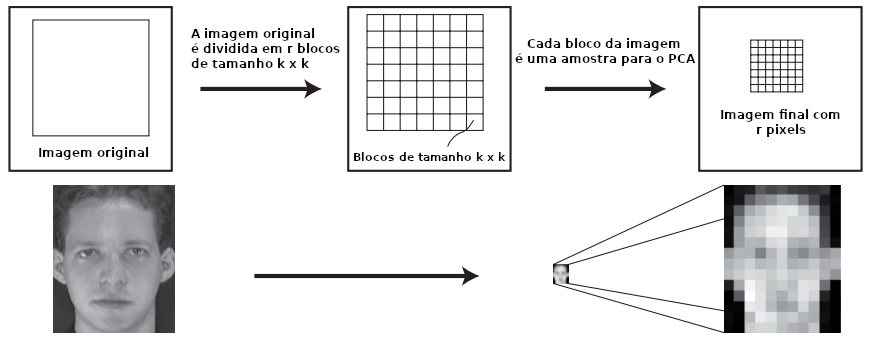
\includegraphics[width=1\textwidth]{recursos/imagens/proposal/BPCA.png}
    \label{proposal:pcapooling:fig:3}

    Fonte: retirado e adaptado de \cite{Salvadeo2011}.
\end{figure}

\paragraph{VGG-16}

\paragraph{U-Net-Like}

\paragraph{U-Net}

\subsection{Metodologia Experimental}
\label{project:exp_result}
O método de avaliação escolhido seguiu no mesmo caminho do artigo tomado como referência para realizar a segmentação \textit{Part-Aware Panoptic Segmentation} \cite{DeGeus2021}, que, no que lhe concerne, teve como base o artigo pioneiro de segmentação panóptica \cite{Kirillov2019a}, que aplica a métrica PQ (Equação \ref{panoptic:eq:2}), realizando uma sucinta adaptação que possibilita quantificar as partes das segmentações panópticas visto que é aplicado para cada uma das classes ($l$) presentes na cena, sendo elas \textit{thing} ou \textit{stuff}. Através da equação \ref{proposal:avaliation:eq:1} é possível entender a métrica de avaliação \textit{Part-PQ}, a qual fora escolhida para avaliação:

\begin{equation}
\label{proposal:avaliation:eq:1}
    PartPQ = \frac{\sum _{(p,g) \in VP} IoU_p(p,g)}{|VP|+ \frac{1}{2}|FP| + \frac{1}{2}|FN|}.
\end{equation}

Em relação à Equação \ref{proposal:avaliation:eq:1}, destaca-se ainda que a segmentação das partes dentro de um segmento é capturada principalmente por meio do termo $IoU_p(p,g)$, sendo que no termo é aplicado um condicional com o intuito de deixar a classe segmentada com parte ($\mathcal{L}^{parts}$) e sem partes ($\mathcal{L}^{no-parts}$) dentro das mesmas condições, ou seja, para as classes com partes presentes, aplica-se a métrica de $mIoU$ para cada pixel de parte dentro de um segmento, enquanto para segmentações sem partes, aplica-se a $IoU$ que comumente é utilizada na métrica PQ (Equação \ref{panoptic:eq:2}). O condicional supracitado dá-se por meio da seguinte expressão:

\begin{equation}
\label{proposal:avaliation:eq:2}
    IoU_p(p,g)= \left\{\begin{matrix}
        mIoU_{part}(p,g), & l \in \mathcal{L}^{parts}    & \\ 
        IoU_{ins}(p,g),        & l \in \mathcal{L}^{no-parts} & 
    \end{matrix}\right.
\end{equation}

Por fim, após a aplicação de PartPQ em todas as classes, calcula-se a média entre avaliações realizadas, de modo que é possível avaliar o desempenho do modelo em toda a cena e demonstrou resultados consideráveis quando comparado à métrica original \cite{DeGeus2021}.

\subsubsection{Comportamento das Métricas}

\subsubsection{Explicação de Modelos}


\subsection{Revisão de Literatura}
\label{proposal:revision}
Em meio a vários estilos de revisão, vale dizer que a revisão sistemática é amplamente difundida em meio cientifico, destacando-se em pesquisas de âmbito clínico e médico e garantindo menos viés, maior confiabilidade e um resumo de forma crítica dos trabalhos científicos \cite{barbosa2019}. Sendo assim, no presente trabalho, foi realizada uma revisão, bem como buscas baseadas nos artigos \cite{barbosa2019} e \cite{liberati2009}, de modo que se inspirou nas recomendações dos mesmos, salvo os casos relacionados a questões de aplicações clínicas.

Em relação às revisões, foram realizadas duas, de modo a abranger tanto os artigos técnicos em relação à segmentação panóptica, quanto artigos que servissem de base para a segmentação na área odontológica. A questão a ser tomada como base para esse estudo é: Como projetar um arcabouço para segmentar imagens de componentes visuais hierarquicamente?

Para a primeira revisão citada, foram procurados todo tipo de estudo publicados a partir do ano de 2019 até o ano presente (2022) com o assunto relacionado a \textit{panoptic segmentation}, de modo a se basear no ano de publicação do artigo pioneiro \cite{Kirillov2019a} no assunto. Foram usados os termos a seguir em diferentes combinações: ``\textit{panoptic segmentation}'', ``\textit{part}'' e ``\textit{part-aware}''. Os idiomas foram restritos à português e inglês.

O critério de inclusão baseou-se em artigos que possuíssem a citação da técnica de segmentação \textit{part-aware}, de modo a contribuir com uma segmentação hierárquica dos componentes que compunham a cena. Já em relação aos critérios de exclusão destaca-se artigos com descrição inadequada em relação ao interesse dessa revisão. Quando o artigo era específico para uma determinada aplicação que não condizia com o tema (como carros autônomos) e quando o estudo estava duplicado entre as ferramentas de busca.

Sendo assim, os indicadores referentes às pesquisas realizadas sobre esse assunto podem ser visualizadas no diagrama abaixo (Figura \ref{proposal:revision:fig:1}).

\begin{figure}[H]
    \centering
    \caption{Diagrama de revisão de estudos em segmentação panóptica.}
    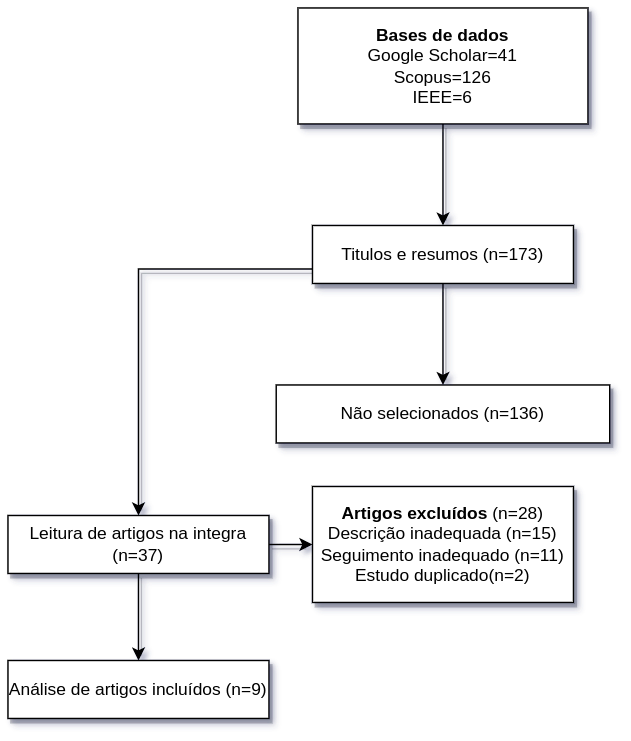
\includegraphics[height=4.5in]{recursos/imagens/proposal/revisao_panoptica.png}
    \label{proposal:revision:fig:1}

    Fonte: do próprio autor.
\end{figure}

Sendo assim, por meio do estudo realizado em relação às referências de segmentação panóptica apenas nove foram escolhidos, para complementar o presente estudo, como demonstrado na Figura \ref{proposal:revision:fig:1}, os quais são listados na Tabela \ref{proposal:revision:tab:1}.

\begin{table}[H]
    \centering
    \caption{Trabalhos selecionados a partir da revisão sobre segmentação panóptica.}
    \label{proposal:revision:tab:1}
    \resizebox{\textwidth}{!}{
    \begin{tabular}{l|l}
        \textbf{Título}                                                &  \textbf{Referência}    \\ \hline
        Part-Aware Panoptic Segmentation                               &  \cite{DeGeus2021}      \\
        Improving Panoptic Segmentation at All Scales                  &  \cite{Porzi2021}       \\
        SpatialFlow: Bridging All Tasks for Panoptic Segmentation      &  \cite{Chen2019a}       \\
        Visual relation of interest detection based on part detection  &  \cite{YouZhou2021}     \\
        Panoptic Image Annotation with a Collaborative Assistant       &  \cite{Jasper2020}      \\
        Panoptic Segmentation-Based Attention for Image Captioning     &  \cite{Cai2020}         \\
        Supplementary Material: Part-aware Panoptic Segmentation       &  \cite{DeGeus2021a}     \\
        Panoptic Segmentation: A Review                                &  \cite{Elharrouss2021}  \\
        PartImageNet: A Large, High-Quality Dataset of Parts           &  \cite{He2021}   
    \end{tabular}}

    \vspace*{1 cm}
    Fonte: do próprio autor.
\end{table}

Quando se trata da segunda revisão em pauta, a que contempla as segmentações na área odontológica, destaca-se que os estudos procurados também não se limitaram ao tipo, incluindo congressos, artigos de revista, entre outros, além de utilizarem o intervalo dos anos de 2019 a 2022 como métrica, de modo a encontrar segmentações odontológicas que acompanhassem a técnica de segmentação panóptica. Os termos utilizados estão listados a seguir, de modo que foram buscados em diferentes combinações: ``odonto'', ``\textit{dentistry}'', ``\textit{deep learning}'', ``\textit{semantic segmentation}'', ``\textit{instance segmentation}'', ``\textit{panoptic segmentation}'' e ``CNN''. Os idiomas foram restritos à português e inglês.

Quanto aos critérios de inclusão, destaca-se os artigos que abordaram ao menos uma das segmentações modernas, de feitio a estarem alinhados com a proposta do projeto. Quanto aos critérios de exclusão, pode-se dizer que são similares aos da primeira revisão, relatando artigos com descrição inadequada acerca da revisão em questão, estudos duplicados entre as ferramentas de busca e quando o estudo não estava diretamente relacionado aos temas ``segmentação'' e ``odontologia''. Dessa forma, por meio da Figura \ref{proposal:revision:fig:2} é possível visualizar a representação da revisão realizada.

\begin{figure}[H]
    \centering
    \caption{Diagrama de revisão de estudos em segmentação odontológica.}
    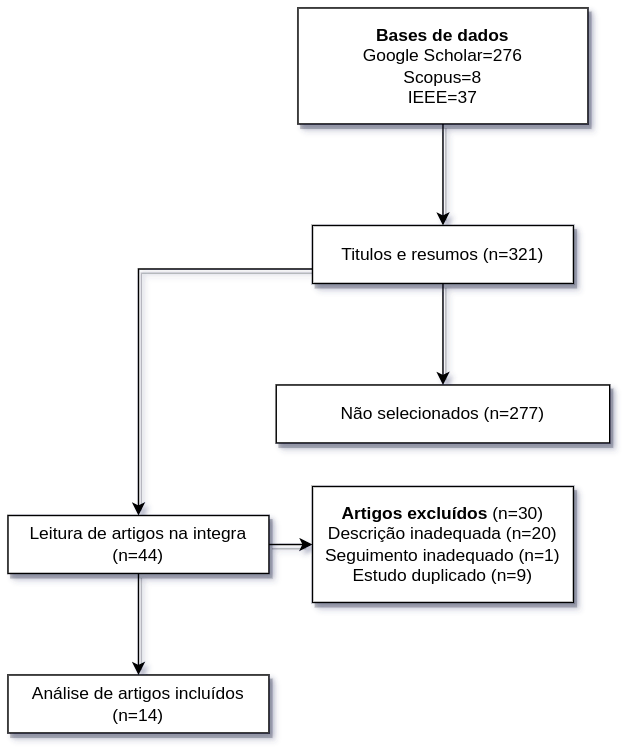
\includegraphics[height=4.5in]{recursos/imagens/proposal/revisao_odonto.png}
    \label{proposal:revision:fig:2}


    Fonte: do próprio autor.
\end{figure}

Tendo em vista os estudos que estão relacionados à segmentação na área odontológica, destacando aqueles que fazem uso das segmentações modernas (semântica, de instâncias ou panóptica), por meio da Figura \ref{proposal:revision:fig:2} cita-se que apenas 14 foram determinados como relevantes, os quais são listados na Tabela \ref{proposal:revision:tab:2}.

\begin{table}[H]
    \centering
    \caption{Trabalhos selecionados a partir da revisão sobre segmentação odontológica.}
    \label{proposal:revision:tab:2}
    \resizebox{\textwidth}{!}{
    \begin{tabular}{l|l}
        \textbf{Título}                                                                                                              &  \textbf{Referência}  \\ \hline
        A study on tooth segmentation and numbering using end-to-end deep neural networks                                            &  \cite{Silva2020}       \\
        Accurate Segmentation of Dental Panoramic Radiographs with U-NETS                                                            &  \cite{Koch2019}        \\
        ToothNet: Automatic Tooth Instance Segmentation and Identification From Cone Beam CT Images                                  &  \cite{Cui2019}         \\
        Toothpix: Pixel-Level Tooth Segmentation in Panoramic X-Ray Images based on Generative Adversarial Networks                  &  \cite{Cui2021}         \\
        Simultaneous Nuclear Instance and Layer Segmentation in Oral Epithelial Dysplasia                                            &  \cite{Shephard2021}    \\
        Automated detection and classification of oral lesions using deep learning to detect oral potentially malignant disorders    &  \cite{Tanriver2021}    \\
        Pose-aware instance segmentation framework from cone beam CT images for tooth segmentation                                   &  \cite{Minyoung2020}    \\
        Mask-MCNet: Instance Segmentation in 3D Point Cloud of Intra-oral Scans                                                      &  \cite{Ghazvinian2021}  \\
        Artificial Intelligence for Fast and Accurate 3-Dimensional Tooth Segmentation on Cone-beam Computed Tomography              &  \cite{Lahoud2021}      \\
        Clinically Applicable System For 3D Teeth Segmentation in Intraoral Scans using Deep Learning                                &  \cite{Hao2020}         \\
        Machine learning in orthodontics: Challenges and perspectives                                                                &  \cite{Liu2021}         \\
        Automatic 3D tooth segmentation using convolutional neural networks in harmonic parameter space                              &  \cite{Zhang2020}       \\
        Automatic Dental Plaque Segmentation based on Local-to-global Features Fused Self-attention Network                          &  \cite{Li2022}          \\
        Interpretable and Interactive Deep Multiple Instance Learning for Dental Caries Classification in Bitewing X-rays            &  \cite{Bergner2021}  
    \end{tabular}}

    \vspace*{1cm}
    Fonte: do próprio autor.
\end{table}

\subsection{Considerações Finais do Capítulo}